\documentclass[titlepage]{article}

\usepackage{graphicx} % for embedding pictures
\usepackage{wrapfig} % for use with figures
\usepackage[hidelinks]{hyperref} % allows embedding links
\usepackage[dvipsnames]{xcolor} % gives me some colours by name
\usepackage[T1]{fontenc} % fixes weird font size/encoding issues
\usepackage{listings} % used to format code
\usepackage{algorithm} % used with the below package to format psuedo code
\usepackage[noend]{algpseudocode}
\usepackage{mathtools} % used for all the mathematical notation
\usepackage{etaremune} % enumerate backwards for OSI model
\usepackage{placeins} % used to ensure everything stays inside where it is 
% defined, i.e. subsections jumping above figures etc.
\usepackage[nopostdot]{glossaries} % guess what. It manages glossaries
\setacronymstyle{long-short}
\makenoidxglossaries{}

\loadglsentries{glossary}

\definecolor{dkgreen}{rgb}{0,0.6,0}
\definecolor{gray}{rgb}{0.5,0.5,0.5}
\definecolor{mauve}{rgb}{0.58,0,0.82}

% code formatting options
\lstset{%
  frame=tb,
  showstringspaces=false,
  columns=flexible,
  basicstyle={\small\ttfamily},
  numbers=left,
  numberstyle=\tiny\color{gray},
  keywordstyle=\color{blue},
  commentstyle=\color{dkgreen},
  stringstyle=\color{mauve},
  breaklines=true,
  breakatwhitespace=true
}


% forces [sub]sections to contain everything that is defined before the next one
\let\Oldsection\section{}
\renewcommand{\section}{\FloatBarrier\Oldsection}

\let\Oldsubsection\subsection{}
\renewcommand{\subsection}{\FloatBarrier\Oldsubsection}

\let\Oldsubsubsection\subsubsection{}
\renewcommand{\subsubsection}{\FloatBarrier\Oldsubsubsection}


% title
\author{Sam Leonard}
\title{A Level Computer Science Non-Examined Assessment (NEA)}
\date{} % this forces no date to be shown


\begin{document}

\maketitle

\tableofcontents

\section{Analysis}

\subsection{Identification and Background to the Problem (Core)}

The problem I am trying to solve with my project is how to look at devices on a network
from a ``\gls{bbox}'' perspective and gain information about what service are running etc.
There are many steps in-between a device turning on to interacting with the internet.

\begin{enumerate}
  \item{load networking \glspl{driver}}
  \item{Starting \gls{dhcp} \gls{daemon}}
  \item{Broadcasting \gls{dhcp} request for an \gls{ipaddr}}
  \item{Get assigned an \gls{ipaddr}}
  \item{???}
  \item{Profit!!!}
\end{enumerate}

There are many more steps than I have listed above. Starting from a linux computer being switched on
the first step is that the \gls{kernel} needs to load the networking \glspl{driver}. The \gls{kernel} is the basis for the
operating system, it is what interacts with the hardware in the most fundamental way. \glspl{driver} are small
bits of code which the \gls{kernel} can load in order to interact with certain hardware modules such as the
\gls{nic} which is essential for interfacing with the network, hence the name.

Next once the \gls{kernel} has loaded the required \glspl{driver} and the system has booted the networking
`\glspl{daemon}' must be started. In linux a \gls{daemon} is a program that runs all the time in the background
to serve a specific purpose or utility. For example when I start my laptop the following \glspl{daemon} start
\gls{upow} (power management), \gls{sysd} (manages the creation of all processes), \gls{dbus} (manages
inter-process communication), iwd (manages my WiFi connections) and finally \gls{dhcpcd} which manages all
interactions with the network around \gls{dhcp}.

Once the \glspl{daemon} are all started the \gls{dhcp} client sends a discover message with the address
255.255.255.255 which is the IP limited broadcast address which means that whatever is listening at the
other end will forward this packet on to everyone on the \gls{subnet}. When the \gls{dhcp} \gls{server} on the subnet
receives this message it reserves a free \gls{ipaddr} for that client and then responds with a \gls{dhcp} offer
which contains the address the \gls{server} is offering, the length of time the address is valid for and the
\gls{subnet} mask of the network. The client must then respond with a \gls{dhcp} request message to request the
offered address, this is in case of multiple DHCP servers offering addresses. Finally the \gls{dhcp} server responds
with a \gls{dhcp} acknowledge message showing that it has received the request. Figure~\ref{dhcp_negotiate} shows
a packet capture from my laptop where I turned WiFi off, started wireshark listening and plugged in an Ethernet
cable, I have it showing only the \gls{dhcp} packets so that it is clear to see the entire \gls{dhcp} negotiation
including the 255.255.255.255 limited broadcast destination address and the 0.0.0.0 unassigned address in the source
column.

\begin{figure}[H]
  \centering
  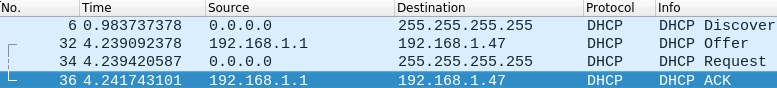
\includegraphics[width=\textwidth]{screenshots/dhcp_negotiation.png}
  \caption{\gls{dhcp} address negotiation}\label{dhcp_negotiate}
\end{figure}

All computer networking is encapsulated in the \gls{osi} which has 7 layers:
\begin{etaremune}
  \item{Application: \gls{api}s, \gls{http}, \gls{ftp} among others.}
  \item{Presentation: encryption/decryption, encoding/decoding, decompression etc\ldots}
  \item{Session: Managing sessions, \gls{php} session IDs etc\ldots}
  \item{Transport: TCP and UDP among others.}
  \item{Network: ICMP and IP among others.}
  \item{Data Link: MAC addressing, Ethernet protocol etc\ldots}
  \item{Physical: The physical Ethernet cabling/\gls{nic}.}
\end{etaremune}
Each of these layers is essential to the running of the internet but a single communication
might not include all of the layers. I'm going to use the example of getting a very
simple static HTML page with an image inside. The code for the page is shown in
listing~\ref{examplepage}. In figure~\ref{basicwebpage} you can see how the page renders.
However far more interestingly is how the browser retrieved the page, in figure~\ref{getrequest}
you can see the full sequence of packets that were exchanged for the browser to get the resources
it needed to render the page. I am hosting the page using python3's http.server module
which is super convenient and just makes the current directory open on 127.0.0.1 port 8000
from there I can just navigate to /example.html and it will render the page. Breaking
figure~\ref{getrequest} down packet one shows the browser receiving the request from
the user to display \verb|http://127.0.0.1:8000/example.html| and attempting to connect
to 127.0.0.1 on port 8000. Packets two and three show the negotiation of this request
through to the full connection being made. The browser now makes an \gls{http} GET
request for the page example.html over the established TCP connection as shown in packet 4.
The server then acknowledges the request and sends a packet with the PSH flag set
as shown in packets 6 and 7. The PSH flag is a request to the browser to say that it is
OK to received the buffered data, i.e.\ example.html. The browser then sends back an
acknowledgement and the server sends the page as shown in packets 7 and 8. Finally
the browser sends a final acknowledgement of having received the page before initiating
a graceful session teardown by sending a FIN ACK packet which indicates the end of a session.
Once the server responds to the FIN ACK with it's own the browser sends a final acknowledgement.
This then repeats itself when the browser parses the HTML and realises theres an image which
it needs to get from the server as well, except the image is a larger file and so takes a few
more PSH packets.

This shows clearly the interaction between each of the different layers in the OSI model,
the browser at level 7: Application rendering the webpage. Level 6: Presentation is skipped as
we have no files which need to be served compressed because they are so large. Level 5: Session
is shown by the TCP session negotiation and graceful teardown of the TCP session. Level 4: Transport
is shown when the image and webpage are transferred from the server to the browser. Level 3/2/1
are shown in figure~\ref{deconstructed} where you can see the IP layer information along with
Ethernet II and finally frame 4 which is the bytes that went down the wire.


\begin{figure}[H]
  \centering
  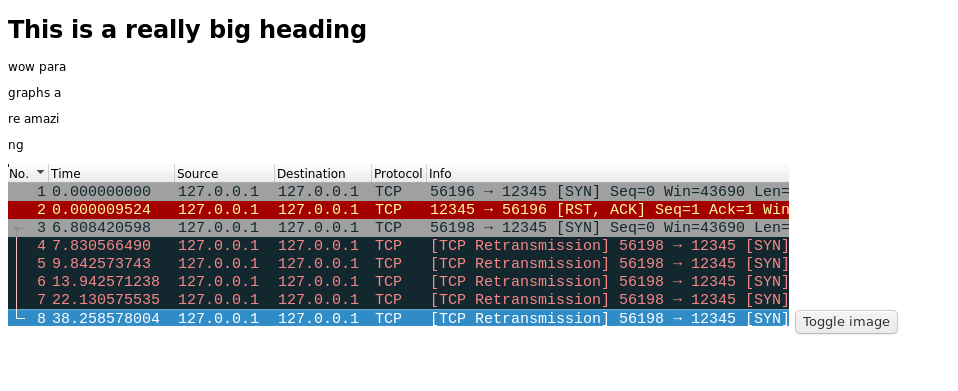
\includegraphics[width=\textwidth]{screenshots/basic_webpage.png}
  \caption{%
    A basic static \gls{html} webpage.
  }\label{basicwebpage}
\end{figure}

\begin{figure}[H]
  \centering
  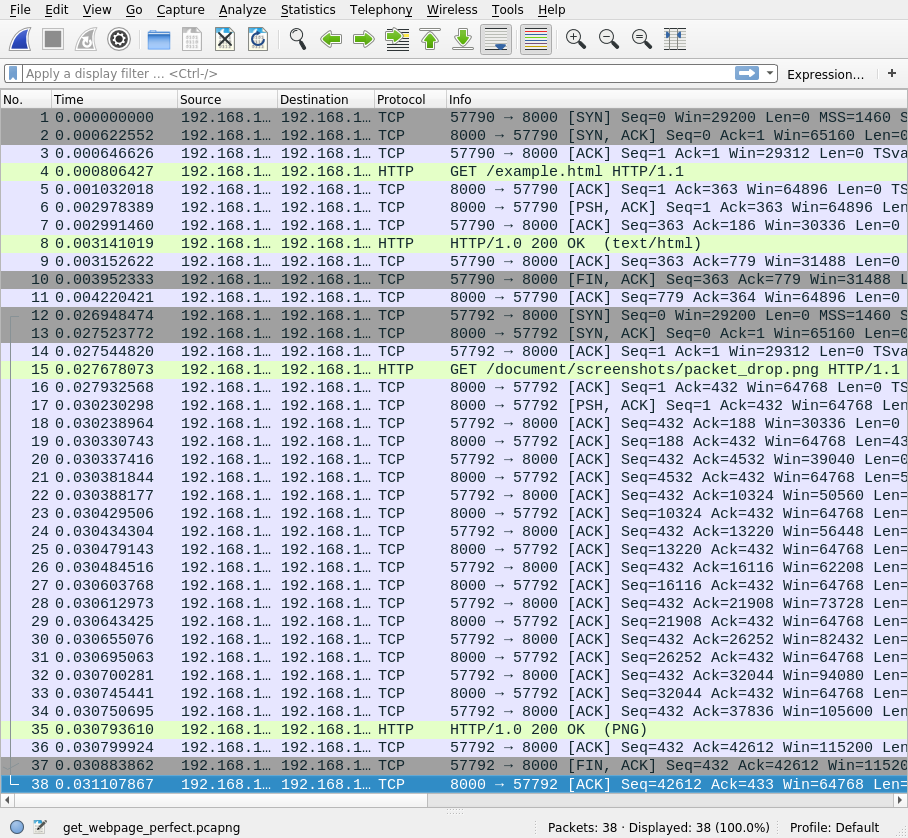
\includegraphics[width=\textwidth]{screenshots/website_get.png}
  \caption{%
    A full chain of packets that shows retrieving a basic webpage
    from the server.
  }\label{getrequest}
\end{figure}

\begin{figure}[H]
  \centering
  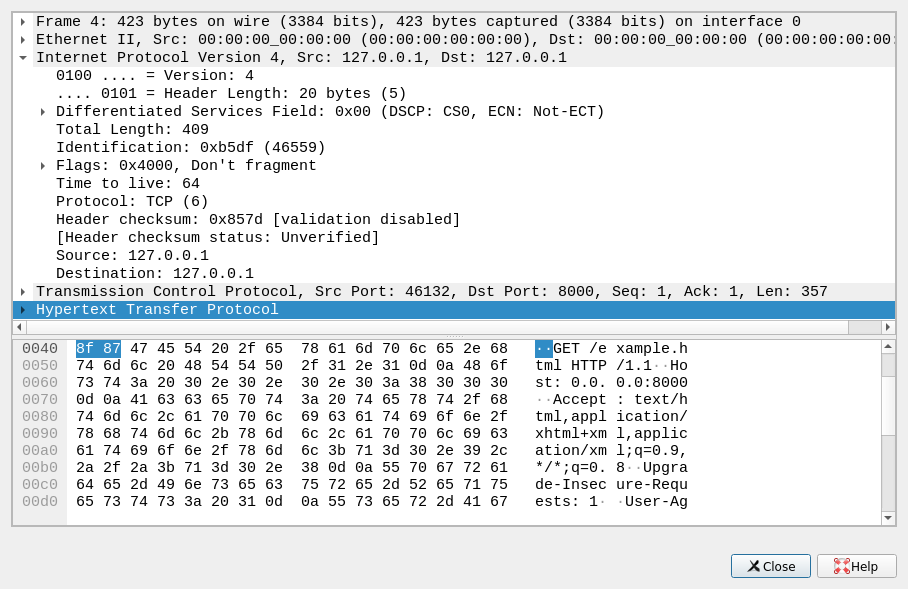
\includegraphics[width=\textwidth]{screenshots/deconstructed_packet.png}
  \caption{%
    A look inside a TCP packet.
  }\label{deconstructed}
\end{figure}

\lstset{language=HTML}
\lstinputlisting[caption={example.html}, label={examplepage}]{../example.html}

\subsection{Analysis of problem (Core)}

The problem with looking at a network from the outside is that the purpose of the network is to
allow communication inside of the network, thus very little is exposed externally. This presents
a challenge as we want to know what is on the network as well as what each of them is running which
is not always possible due to the limited information that services will reveal about themselves.
Firewalls also play large part in making scanning networks difficult as sometimes they simply drop
\glspl{pkt} instead of sending a \gls{tcp} RST \gls{pkt} (reset connection \gls{pkt}).
When firewalls drop \glspl{pkt} it becomes exponentially more difficult as you don't know whether
your \gls{pkt} was corrupted or lost in transit or if it was just dropped.

In figure~\ref{firewall} you can see the difference between trying to connect to a closed port
when there is no rule saying to drop packets and when I introduce a rule to drop packets.
The first packet at time zero shows the connection request on line \verb%In [3]% of
figure~\ref{firewall_code} then nine microseconds later a RST, ACK packet is sent back
showing the port is closed as shown in figure~\ref{firewall_code} by the
\verb$ConnectionRefusedError$ that the socket module throws when we try to connect to a closed
port. Packet number three in figure~\ref{firewall} shows the connection request from \verb|In [4]|
except that I have enabled a firewall rule to drop all packets from the address 127.0.0.1, using
the iptables command as so: \verb$iptables -I INPUT -s 127.0.0.1 -j DROP$. This command reads
as for all packets arriving (\verb|-I INPUT|) with source address 127.0.0.1 (\verb|-s 127.0.0.1|)
drop them sending no response (\verb|-j DROP|). With this firewall rule in place you can see in
figure~\ref{firewall} packet 3 receives no response and as such python assumes that the packet
just got lost and as such tries to send the packet again repeatedly, this continued for more than
30 seconds before a stopped it as shown by the time column in figure~\ref{firewall} and the final
\verb|KeyboardInterrupt| in figure~\ref{firewall_code}. The amount of time that a system will wait
still trying to reconnect depends on the OS and a other factors but the minimum time is 100 seconds
as specified by RFC 1122, on most systems it will be between 13 and 30 minutes according the
linux manual page on tcp.
\begin{verbatim}
man 7 tcp:
tcp_retries2 (integer; default: 15; since Linux 2.2)
  The maximum number of times a TCP packet is retransmitted in
  established state before giving up. The default value is 15,
  which corresponds to a duration of approximately between 13 to 30
  minutes, depending on the retransmission timeout. The RFC 1122
  specified minimum limit of 100 seconds is typically deemed too short.
\end{verbatim}

\begin{figure}[H]
  \centering
  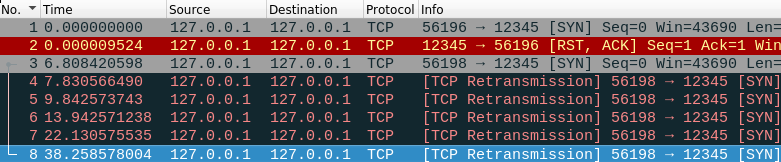
\includegraphics[width=\textwidth]{screenshots/packet_drop.png}
  \caption{%
    Attempted connection to a closed port with and without firewall rule to drop packets.
  }\label{firewall}
\end{figure}

\begin{figure}[H]
  \centering
  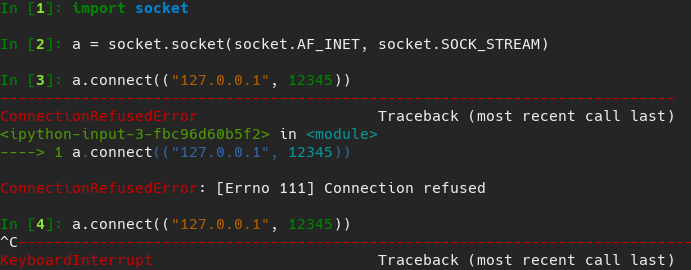
\includegraphics[width=\textwidth]{screenshots/packet_drop_code.png}
  \caption{%
    The code used to produce firewall packet dropping example in figure~\ref{firewall}
  }\label{firewall_code}
\end{figure}

\subsection{Numbered List of Objectives (also called Success Criteria, the end user requirements) (Core)}

\begin{enumerate}
\item{Show a basic usage message when called with no arguments.}
\item{Show a help message when called with \texttt{--help} or \texttt{-h}.}
\item{Scan the 1000 most commonly used \gls{tcp} \glspl{port} when called with just an \gls{ipaddr}.}
\item{Scan the \glspl{port} specified by \texttt{-p <ports>} or \texttt{--ports <ports>}.}
\item{Parse either a comma separated list of \glspl{port} e.g.\ \texttt{1,2,3,4} or a range specified set of \glspl{port} e.g.
  \texttt{1{\textendash}4}}.
\item{Scan all \glspl{port} in each scan type when called with \texttt{-p-}.}
\item{Don't scan the \glspl{port} specified by \texttt{--exclude-ports <ports>} in any scan.}
\item{Expand a \gls{cidr} specified \gls{subnet} when used in the target specification.}
\item{List all of the \gls{ipaddr}es that would be scanned when given the \texttt{-sL} flag.}
\item{Only ping each specified address when supplied the \texttt{-sn} flag.}
\item{When doing a ping scan (\texttt{-sn}) display the Time To Live (TTL) and latency of each host.}
\item{Don't ping each of the hosts before scanning to check if they are up when supplied with the \texttt{-Pn} flag.}
\item{Perform a \gls{tcp}SYN scan on the 1000 most common \gls{tcp} \glspl{port} on each target specified when given the \texttt{-sS} flag.}
\item{Perform a \gls{tcp} \verb|Connect()| scan on the 1000 most common \gls{tcp} \glspl{port} on each target specified when given the \texttt{-sT} flag.}
\item{Perform a\gls{udp}scan on the 1000 most common\gls{udp} \glspl{port} when on each target specified when given the \texttt{-sU} flag.}
\item{Perform version detection on the services running on each of the hosts specific when given the \texttt{-sV} flag.}
\end{enumerate}

\subsection{Description of current system or existing solutions (Core if relevant)}

Nmap is currently the most popular tool for doing\gls{port}scanning and host enumeration.
It supports the following scanning types:

\begin{itemize}
\item{\gls{tcp}:\ SYN}
\item{\gls{tcp}:\ \verb|Connect()|}
\item{\gls{tcp}:\ ACK}
\item{\gls{tcp}:\ Window}
\item{\gls{tcp}:\ Maimon}
\item{\gls{tcp}:\ Null}
\item{\gls{tcp}:\ FIN}
\item{\gls{tcp}:\ Xmas}
\item{\gls{udp}}
\item{Zombie host/idle}
\item{\gls{sctp}:\ INIT}
\item{\gls{sctp}:\ COOKIE-ECHO}
\item{IP protocol scan}
\item{\gls{ftp}:\ bounce scan}
\end{itemize}

As well as supporting a vast array of scanning types it also can do service version detection
and operating system detection via custom probes. Nmap also has script scanning which allows
the user to write a script specifying exactly how they want to scan e.g.\ to circumvent \gls{port knocking}
(where \glspl{pkt} must be sent to a sequence of \glspl{port} in order before access to the final\gls{port}is allowed).
It also supports a plethora of options to avoid firewalls or \gls{ids} such as sending
\glspl{pkt} with spoofed \glspl{csum}/source addresses and sending decoy probes. Nmap can do many more things than I
have listed above as is illustrated quite clearly by the fact there is an entire working on using nmap
(\href{https://nmap.org/book/}{https://nmap.org/book/})

\subsection{Prospective Users (Desirable)}

The prospective users of this system would be system administrators, penetration testers or network engineers.
In my case my prospective users would be my school's system administrators and it would allow them to see an
outsiders perspective on for example the \gls{server} running the school's website page or to see if any of the
programs on the \glspl{server} were leaking information through \glspl{banner} etc. (most services send a \gls{banner} with
information like what protocol version they use and other information)

\subsection{Data Dictionary (Desirable)}

\textbf{\color{red}{I looked this up and it seemed to be related to database management systems.}}

\href{https://en.wikipedia.org/wiki/Data_dictionary}{https://en.wikipedia.org/wiki/Data\_dictionary}

\subsection{Data Flow Diagram (Desirable)}

\textbf{\color{red}{This seems to be fairly relevant and to do with how data goes through my program
    i.e.\ going from the network to my port scanner into a target object and other scanners
before version detection and finally displaying to the user. Make a flowchart for this.}}

\href{https://en.wikipedia.org/wiki/Data-flow_diagram<Paste>}{https://en.wikipedia.org/wiki/Data-flow\_diagram}

\subsection{Data Sources (Desirable)}

\textbf{\color{red}{Not really sure about this.}}

\subsection{Description of Solution Details, OOP/Mobile/Networking (Core if relevant)}

To do all forms of scanning other than \verb|Connect()| scanning and version detection, custom
\glspl{pkt} are made to allow the \gls{half open} (no full connection is made to the host) scanning
used in\gls{tcp}SYN scanning. Making custom \glspl{pkt} is quite difficult because the endianness
(the order the bytes are interpreted in: big endian, most significant byte first, little endian,
least significant byte first) affects how all the information packed into the \gls{pkt} is interpreted
by the network switch, for example the\gls{ipaddr}192.168.1.58 packed in big endian form but interpreted
being in little endian form comes out as 58.1.168.192 which is a completely different address and
will mean the \gls{pkt} is not routed to the correct host. As well as the issues with byte order
and the interpretation of information at different points the \gls{csum} which is embedded into
the \gls{pkt} is calculated from a psuedo-header calculated from information in the underlying
IP header and all of this has to be calculated in the right byte order (endianness).

I have used Python's multiprocessing module to allow me to spawn another process which listens
for responses from hosts and waits for a certain amount of time before returning information
on what hosts responded and in the case of ping scanning also metadata about how they responded.

In version detection scanning the relationship between the data sources and modules used is quite
complex so I have used an \gls{oop} approach to group the methods
that act on the data along with the data itself. For example each probe defined in the nmap-service-probes
file can be sent to a host and matched against a list of match directives stored in the probe,
the probe class has a scan method which sends it's probe to the host and then automatically runs
match and soft-match directives against the information returned by the probe.

Parsing the match and softmatch directives was quite difficult because they include regular
expressions with special characters such as newlines and carriage returns in the form of
\verb|\n| and \verb|\r| characters which python escapes to \verb|\\n|
and \verb|\\r|. Which instead of matching a newline character and a carriage return
will match a literal backslash and then an n or an r which is not what we want. To fix this I have to substitute
newline and carriage returns back in where I find \verb|\\r| and \verb|\\r|.

\subsection{Acceptable Limitations (Supplementary)}

Originally I had planned to include dedicated operating system detection as an option
however I ran out of time having implemented version detection. However it still does
Operating system detection partially as some services are linux only and while doing
service and version detection especially the \gls{cpe} parts
of the matched service/version will contain operating system information, such as
microsoft ActiveSync would indicate that the system being scanned was a windows system
which is reflected in the match directive and attached CPE information: \texttt{%
match activesync m|{\textasciicircum}.{\textbackslash}0{\textbackslash}x01{\textbackslash}0[{\textasciicircum}{\textbackslash}0]{\textbackslash}0[{\textasciicircum}{\textbackslash}0]{\textbackslash}0[{\textasciicircum}{\textbackslash}0]{\textbackslash}0[{\textasciicircum}{\textbackslash}0]{\textbackslash}0[{\textasciicircum}{\textbackslash}0]{\textbackslash}0.*{\textbackslash}0{\textbackslash}0{\textbackslash}0\$|s p/Microsoft ActiveSync/ o/Windows/ cpe:/a:microsoft:activesync/ cpe:/o:microsoft:windows/a
}


\subsection{Data Volumes (Supplementary)}

\textbf{\color{red}{This seems to be about the volume of data stored in a database.}}
\href{https://stackoverflow.com/questions/5566841/what-are-data-volumes#5567390}{https://stackoverflow.com/questions/5566841/what-are-data-volumes\#5567390}

\subsection{Test Strategy (Core)}

I am going to use two different methods to test my program:
\begin{enumerate}
\item{Unit testing}
\item{Wireshark}
\end{enumerate}
I am using two separate testing strategies because they are both good at different things,
both of which I need to show that my project works. Firstly I am using unit testing to test
some general purpose functions which are pure functions (are independent of the current state
of the machine) such as \verb|ip_range()| and other functions which I can
just check the returned value against what it should be.

Wireshark is useful for the other half of the program which uses impure functions and the
low level networking e.g.\ \verb|make_tcp_packet()|. Wireshark makes this easy by allowing capture of all
the \glspl{pkt} going over the wire, as well as this it has a vast array of \gls{pkt} decoders (2231 in my install)
which it can use to dissect almost any \gls{pkt} that would be on the network. The main
benefit of wireshark is that I can see my scanners sending \glspl{pkt} and then check whether the parsers
that I have written for the different protocols are working. I can also check that the \glspl{csum}
in each of the various protocols is valid as wireshark does \gls{csum} verification for various protocols.

\section{Design}

\subsection{Overall System Design (High Level Overview) (Core)}

There are two types of scanning implemented for different scan types in my program.
\begin{itemize}
  \item{\verb|Connect()|}
  \item{version}
  \item{listener / sender}
\end{itemize}
\verb|Connect()| scanning is the simplest in that it takes in a list of \glspl{port} and simply calls the
\verb|socket.connect()| method on it and sees whether it can connect or not and the \glspl{port} are
marked accordingly as open or closed.

Version scanning is very similar to \verb|Connect()| scanning in that it takes in a list of \glspl{port}
and connects to them, except it then sends a probe to the target to elicit a response and gain
some information about the service running behind the \gls{port}.

Listener / sender scanning does exactly what it says on the tin: it sets up a ``listener'' in another process
to listen for responses from the host which the ``sender'' is sending \glspl{pkt} to. It can then differentiate
between open, open|filtered, filtered and closed \glspl{port} based on whether it receives a \gls{pkt} back
and what flags (part of\gls{tcp} \glspl{pkt} are a one byte long section which store ``flags'' where each bit in the
byte represents a different flag) are set in the received \gls{pkt}.

\subsection{Design of User Interfaces HCI (Core)}

I have designed my system to have a similar interface to the most common tool currently used: nmap
this is because I believe that having a familiar interface will not only make it easier for someone who
is familiar with nmap to use my tool it also makes it so that anything learnt using either tool is applicable
to both which benefits everyone.

Based on this perception I have used the same option flags as nmap as well as similar help messages
and an identical call signature (how the program is used on the command line). Running 
\verb|./netscan.py <options> <target_spec>| is identical to \verb|nmap <options> <target_spec>| in terms
of which scan types will be run, which hosts will be scanned and which \glspl{port} are scanned. Below you can see
the help message generated by \verb|./netscan.py --help|.
\begin{verbatim}
usage: netscan.py [-h] [-Pn] [-sL] [-sn] [-sS] [-sT] [-sU] [-sV] [-p PORTS]
                  [--exclude_ports EXCLUDE_PORTS]
                  target_spec

positional arguments:
  target_spec           specify what to scan, i.e. 192.168.1.0/24

optional arguments:
  -h, --help            show this help message and exit
  -Pn                   assume hosts are up
  -sL                   list targets
  -sn                   disable port scanning
  -sS                   TCP SYN scan
  -sT                   TCP connect scan
  -sU                   UDP scan
  -sV                   version scan
  -p PORTS, --ports PORTS
                        scan specified ports
  --exclude_ports EXCLUDE_PORTS
                        ports to exclude from the scan
\end{verbatim}

It shows clearly which are required arguments and which are optional ones, as well as what
each argument actually does. It also allows some some arguments to be called with either
a short format e.g.\ \verb|-p| and with a most verbose format \verb|--ports| this allows
the user to be clearer if they are using the tool as part of an automated script to perform
scanning as it is more immediately obvious what the more verbose flags do.

\subsection{Database Structure (ERD, Normalisation) (Core, if relevant)}

\textbf{\color{red}{I am fairly sure this is irrelevant to mine?}}

\subsection{System Algorithms (Flowcharts) (Core)}

\textbf{\color{Emerald}{When I have finished the first draft of the text bits I will add pictures / flowcharts}}

\subsection{Input data Validation (Core)}

My program takes very little input from the user which means that there is a very low chance of the program
crashing due to user input error as the errors are detected
All data which is entered is either parsed using a regular expression with the case of the
\glspl{port} directive (\verb|-p|) or is run through checking functions like \verb|ip_utils.is_valid_ip|.
As well as using these checking functions whenever an\gls{ipaddr}is converted between ``long form''
and ``dot form'' which is used in every type of scanning.

\subsection{Proposed Algorithms for complex structures (flow charts or Pseudo Code)}

\begin{algorithm}
  \caption{%
  My algorithm for turning a \gls{cidr} specified \gls{subnet} into a list of actual \gls{ipaddr}es
}\label{ip_range}
  \begin{algorithmic}[1]
    \Procedure{ip\_range}{}
    \State{$\textit{network\_bits} \gets \text{number of network bits specified}$}
    \State{$\textit{ip} \gets \text{base IP address}$}
    \State{$\textit{mask} \gets 0$}
    \For{$\textit{maskbit} \gets (32-\textit{network\_bits}),31$}
      \State{$\textit{mask} \gets \textit{mask} + 2^\textit{maskbit}$}
    \EndFor{}
    \State{$\textit{lower\_bound} \gets \text{\textit{ip} AND \textit{mask}}$}
    \Comment{zero the last 32-\textit{network\_bits}}
    \State{$\textit{upper\_bound} \gets \text{\textit{ip} OR (\textit{mask} XOR 0xFFFFFFFF)}$}
    \Comment{turn the last 32-\textit{network\_bits} to ones}
    \State{$\textit{addresses} \gets \text{empty list}$}
    \For{$\textit{address} \gets \textit{lower\_bound},\textit{upper\_bound}$}
      \State{append \Call{convert\_to\_dot}{\textit{address}} to \textit{addresses}}
    \EndFor{}
    \Return{\textit{addresses}}
    \EndProcedure{}
  \end{algorithmic}
\end{algorithm}

\begin{algorithm}
  \caption{%
    My algorithm for pretty-printing a dictionary of lists of\gls{port}numbers
    such that ranges are specified as start-end instead of start,start+1,\ldots,end
  }\label{collapse}
  \begin{algorithmic}[1]
  \Procedure{collapse}{}
    \State{$\textit{port\_dictionary} \gets \text{dictionary of lists of\gls{port}numbers}$}
    \State{$\textit{key\_results} \gets \text{empty list}$}
    \Comment{stores the formatted result for each key}
    \For{\textit{key} in \textit{port\_dictionary}}
      \State{$\textit{ports} \gets \text{\textit{port\_dict}[\textit{key}]}$}
      \State{$\textit{result} \gets \textit{key} + \text{``:\{''}$}
      \If{\textit{ports} is empty}
        \State{$\textit{new\_sequence} \gets FALSE$}
        \For{$\textit{index} \gets 1,\text{(length of \textit{ports})}-1$}
          \State{$\textit{port} = \text{\textit{ports}[\textit{index}]}$}
          \If{$\textit{index} = 0$}
            \State{$\textit{result} \gets \textit{result} + \textit{ports}[0]$}
            \Comment{append the first element}
            \If{$\text{\textit{ports}[\textit{index}+1]} = \textit{port} + 1$}
              \State{$\textit{result} \gets \textit{result}+\text{``-''}$}
              \Comment{begin a new sequence}
            \Else{}
              \State{$\textit{result} \gets \textit{result} + \text{``,''}$}
              \Comment{not a sequence}
            \EndIf{}
          \ElsIf{$\textit{port} + 1 \not= \text{\textit{ports}[\textit{index}+1]}$}
          \Comment{break in sequence}
            \State{$\textit{result} \gets \textit{result} + \textit{port} + \text{``,''}$}
            \State{$\textit{new\_sequence} \gets \textit{TRUE}$}
          \ElsIf{$\textit{port}+1 = \text{\textit{ports}[\textit{index}+1]} \And \textit{new\_sequence}$}
            \State{$\textit{result} \gets \textit{result} + \text{``-''}$}
            \State{$\textit{new\_sequence} \gets \textit{FALSE}$}
          \EndIf{}
        \EndFor{}
      \State{$\textit{result} \gets \textit{result} + \text{\textit{ports}[(length of \textit{ports})-1]} + \text{``\}''}$}
      \State{append \textit{result} to \textit{key\_results}}
      \EndIf{}
    \EndFor{}
    \Return{``\{'' + (\textit{key\_results} separated by ``, '') + ``\}''}
  \EndProcedure{}
  \end{algorithmic}
\end{algorithm}

\subsection{Design Data Dictionary (Core)}

\textbf{\color{red}{I have no idea what this means.
All I can find is that it relates to database structure???}}

\section{Technical Solution}

\subsection{Program Listing} 
\subsection{Comments (Core)}

\subsection{Overview to direct the examiner to areas of complexity and explain design evidence}

\section{Testing}

\subsection{Test Plan}

\subsection{Test Table / Testing Evidence (Core: lots of screenshots)}

\section{Evaluation}

\subsection{Reflection on final outcome}

\subsection{Evaluation against objectives, end user feedback}

\subsection{Potential improvements}

\section{Appendices}

You may show you program listing here

User feedback and survey data

\clearpage
\printnoidxglossaries{}

\end{document}
